%%%%%%%%%%%%%%%%%%%%%%%%%%%%%%%%%%%%%%%%%%%%%%%%%%%%%%%%%%%%%%%%%%%%%%%%%%%%%%%%%%%%%%%%%
%%                                                                                     %%
%%                This file is part of the CAPH Compiler distribution                  %%
%%                            http:%/caph.univ-bpclermont.fr                           %%
%%                                                                                     %%
%%                                  Jocelyn SEROT                                      %%
%%                         Jocelyn.Serot@univ-bpclermont.fr                            %%
%%                                                                                     %%
%%         Copyright 2011-2018 Jocelyn SEROT.  All rights reserved.                    %%
%%  This file is distributed under the terms of the GNU Library General Public License %%
%%      with the special exception on linking described in file ..%LICENSE.            %%
%%                                                                                     %%
%%%%%%%%%%%%%%%%%%%%%%%%%%%%%%%%%%%%%%%%%%%%%%%%%%%%%%%%%%%%%%%%%%%%%%%%%%%%%%%%%%%%%%%%%

\chapter{Dealing with images}
\label{cha:cl-images}

This chapter describes the implementation, simulation and synthesis, using the command-line
interface, of the application based upon the concepts introduced in Chapter~\ref{cha:lang-images}. 

\medskip The code of this application, using the \texttt{inv} actor introduced in
Chapter~\ref{cha:lang-images}, is given in Listing~\ref{lst:invimg-full}. There's only \verb|net|
declaration, instantiating the \verb|inv| actor. The first line (\verb|#include "dc.cph"| is
mandatory for making use of the \verb|dc| type. The input image is to be read in file
\verb|lena128.pgm| and the result to be written in file \verb|result.pgm|\footnote{The PGM (Portable
  Graymap Format) is a portable format for representing gray level images introduced in the NetPBM
  projet~\cite{PGM}. \caph use the P2 (ASCII) sub-format.}.

\begin{lstlisting}[style=CaphStyle,caption={Complete CAPH source code for 
    an application computing negative images},label={lst:invimg-full}]
#include "dc.cph"

actor inv ()
  in (i:unsigned<8> dc)
  out (o:unsigned<8> dc)
rules
| i:'< -> o:'<
| i:'> -> o:'>
| i:'x -> o:'255-x
;

stream inp:unsigned<8> dc from "lena128.pgm";
stream outp:unsigned<8> dc to "result.pgm";

net outp = inv inp;\end{lstlisting}

\medskip
This program can be found in the \verb|examples/primer/invimg| directory in the CAPH distribution.

The corresponding project file (also to be found in the examples directory) is shown in
Listing~\ref{lst:invimg-proj}.  The option \verb|-abbrev-dc-ctors|, at lines 1 and 2, tells the
simulators (interpreter and SystemC-based, respectively) to read and write input and output files
using the abbreviated syntax for control tokens. 

\begin{lstlisting}[style=MakeStyle,caption={File
    \texttt{invimg.proj} for the \texttt{invimg} program of Listing~\ref{lst:invimg-full}},label={lst:invimg-proj}]
SIM_OPTS = -abbrev_dc_ctors
SC_OPTS = -sc_stop_time 1000000 -sc_abbrev_dc_ctors
GHDL_RUN_OPTS = --stop-time=400000ns
\end{lstlisting}

Let's build the top-level Makefile by typing

\begin{lstlisting}[style=BashInputStyle]
# caphmake
\end{lstlisting}

Then, the dataflow graphical representation of the program is easily obtained by invoking 

\begin{lstlisting}[style=BashInputStyle]
# make dot.show
\end{lstlisting}

The representation is shown in Fig.~\ref{fig:inv-dot}

\begin{figure}[htbp]
  \centering
 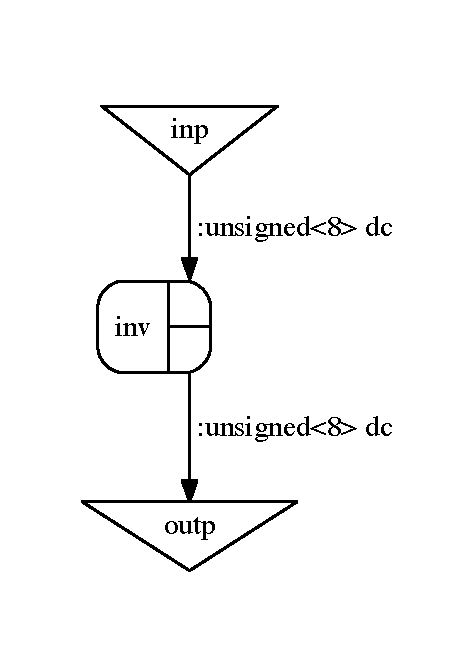
\includegraphics[width=0.3\textwidth]{./figs/inv-dot.pdf}
  \caption{The graphical representation of the program given in Listing.~\ref{lst:invimg-full}}
  \label{fig:inv-dot}
\end{figure}

\section{Simulation}
\label{sec:simulation-2}

The simulator cannot directly read and write images encoded with the PGM format. For this reason,
the CAPH distribution comes with a pair of utility programs, \verb|pgm2txt| and \verb|txt2pgm|, to
convert a PGM~\cite{PGM} file into a structured text file format and \emph{vice-versa} in which
pixels and start/end of line/frame are encoded using the \verb|dc| type introduced in
Chapter~\ref{sec:repr-imag}. A detailed description of these tools can be found in the reference
manual. They programs can called directly from the command line before and after launching the
simulation (to convert from and to the PGM format respectively), but this step can automatized
further by writing a dedicated auxilliary files called a \verb|.procs| file.  In our case, the
contents of this file (also to be found in the \verb|primer/invimg| directory) is reproduced in
Listing~\ref{lst:invimg-procs}.  The first line instructs the compiler to produce the file
\verb|lena128.txt| containing the input image in structured text format, ready for simulation, from
the input image file \verb|lena128.pgm|\footnote{The effect of the \texttt{-abbrev} option is to use
  the abbreviated format (\texttt{<}, \texttt{>}) for d(enoting control and data tokens. Without it,
  these tokens will be written as \texttt{SoS}, \texttt{EoS} and \texttt{Data} respectively.}.  The
second line instructs the compiler to produce the file \verb|result.pgm| containing the result image
in PGM format\footnote{As for \texttt{pgm2txt}, the \texttt{-abbrev} option indicates that the input
  text file uses the abbreviated format for tokens. The numerical argument (255, here) gives the
  maximum value to be written in the PGM file header.}.

\begin{lstlisting}[style=MakeStyle,caption={File
    \texttt{invimg.procs} for the \texttt{invimg} program of
    Listing~\ref{lst:invimg-full}},label={lst:invimg-procs}]
PRE_PROC = pgm2txt -abbrev lena128.pgm lena128.txt
POST_PROC = txt2pgm -abbrev 255 result.txt result.pgm
\end{lstlisting}

\medskip
Simulation is then performed simply by invoking

\begin{lstlisting}[style=BashInputStyle]
# make sim.makefile
# make sim
\end{lstlisting}

This yields the following output 

\begin{lstlisting}[style=BashOutputStyle]
make -f Makefile.sim run CAPH=/usr/local/caph
/usr/local/caph/bin/pgm2txt -abbrev lena128.pgm lena128.txt
/usr/local/caph/bin/caphc -sim -I /usr/local/caph/lib/caph -I /usr/local/caph/lib/caph -abbrev_dc_ctors main.cph
-------------------------------------------------------------------------------------------------
This is the Caph compiler, version 2.8.3
(C) 2011-2017 J. Serot (Jocelyn.Serot@univ-bpclermont.fr)
For more information, see : http://caph.univ-bpclermont.fr
-------------------------------------------------------------------------------------------------
Wrote file ./result.txt
\end{lstlisting}

Viewing the result image is obtained by typing

\begin{lstlisting}[style=BashInputStyle]
# make sim.show
\end{lstlisting}

This invokes the \verb|txt2pgm| utility and launch the PGM image viewing program which has been
specified when installing \caph. In our case, the results are show below and in
Fig.~\ref{fig:inv-result}-b.

\begin{lstlisting}[style=BashOutputStyle]
make -f Makefile.sim show CAPH=/usr/local/caph
/usr/local/caph/bin/txt2pgm -abbrev 255 result.txt result.pgm
open -a Toyviewer result.pgm
\end{lstlisting}

\begin{figure}[htbp]
  \centering
  \begin{tabular}[c]{cc}
 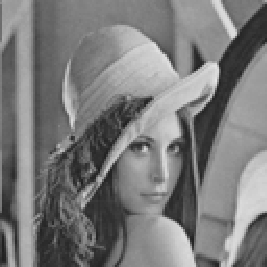
\includegraphics[width=0.3\textwidth]{./figs/lena128.pdf} &
 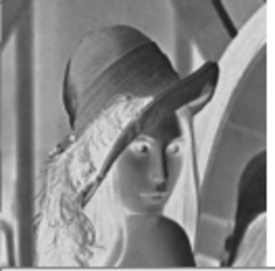
\includegraphics[width=0.3\textwidth]{./figs/inv-result.pdf} \\
 a & b
  \end{tabular}
  \caption{Input and output images after simulation for the program given in Listing.~\ref{lst:invimg-full}}
  \label{fig:inv-result}
\end{figure}

\section{Simulation using the SystemC backend}
\label{sec:simul-using-sysc-2}

As in the previous chapter, this is done by simply typing 

\begin{lstlisting}[style=BashInputStyle]
# make systemc.makefile
# make systemc.run
\end{lstlisting}

Executing this command yields the following output 

\begin{lstlisting}[style=BashOutputStyle]
make -f Makefile.systemc run CAPH=/usr/local/caph
/usr/local/caph/bin/caphc -I /usr/local/caph/lib/caph -systemc -I /usr/local/caph/lib/caph -sc_stop_time 1000000 -sc_abbrev_dc_ctors  main.cph
...
Wrote file ./invimg_expanded.dot
Wrote file ./invimg_net.cpp
Wrote file ./invimg_globals.h
Wrote file ./invimg_globals.cpp
Wrote file ./inv_act.h
Wrote file ./inv_act.cpp
(cd .; g++ -std=c++11 -I. -I/usr/local/caph/lib/systemc ... -c `basename inv_act.cpp`)
(cd .; g++ -std=c++11 -I. -I/usr/local/caph/lib/systemc ... -c `basename invimg_globals.cpp`)
(cd .; g++ -std=c++11 -I. -I/usr/local/caph/lib/systemc ... -c `basename invimg_net.cpp`)
(cd .; g++ -L/usr/local/systemc-2.3.1/lib-macosx64 inv_act.o invimg_globals.o invimg_net.o
   -o invimg_sc -lsystemc  2>&1 | c++filt)
./invimg_sc
        SystemC 2.3.1-Accellera --- Aug  9 2015 15:42:56
        Copyright (c) 1996-2014 by all Contributors,
        ALL RIGHTS RESERVED
Simulation stopped at t=1 ms
\end{lstlisting}

Viewing the file \verb|result.txt| is then handled exactly like above, by invoking 

\begin{lstlisting}[style=BashInputStyle]
# make systemc.show
\end{lstlisting}

\section{Generating and  simulating VHDL code}
\label{sec:generating-vhdl-2}

The process, again, is similar. Simply type

\begin{lstlisting}[style=BashInputStyle]
# make vhdl.makefile
# make vhdl.run
\end{lstlisting}

Executing this command yields the following output 

\begin{lstlisting}[style=BashOutputStyle]
make -f Makefile.vhdl run CAPH=/usr/local/caph
/usr/local/caph/bin/caphc -I /usr/local/caph/lib/caph -vhdl -I /usr/local/caph/lib/caph main.cph
...
Wrote file ./invimg_expanded.dot
Reverting to default size for fifo F5
Reverting to default size for fifo F4
Wrote file ./invimg_net.vhd
Wrote file ./invimg_types.vhd
Wrote file ./inv_act.vhd
Wrote file ./invimg_tb.vhd
warning: VHDL annotation file fifo_caps.dat does not exist.
(cd .; ghdl -a -P/usr/local/caph/lib/vhdl `basename invimg_types.vhd`)
(cd .; ghdl -a -P/usr/local/caph/lib/vhdl `basename invimg_tb.vhd`)
(cd .; ghdl -a -P/usr/local/caph/lib/vhdl `basename inv_act.vhd`)
(cd .; ghdl -a -P/usr/local/caph/lib/vhdl `basename invimg_net.vhd`)
(cd .; ghdl -e -P/usr/local/caph/lib/vhdl invimg_tb)
/usr/local/caph/bin/pgm2bin 8 lena128.pgm lena128.bin
ghdl -r -P/usr/local/caph/lib/vhdl invimg_tb --stop-time=400000ns  
./invimg_tb:info: simulation stopped by --stop-time
\end{lstlisting}

Viewing the file \verb|result.txt| is then handled exactly like above, by invoking 

\begin{lstlisting}[style=BashInputStyle]
# make vhdl.show
\end{lstlisting}

The only difference here with the steps described in the previous section concerns the
generation of the input file(s) and the conversion of the output file(s) to/from the custom
\verb|bin| format used by the VHDL simulator. The utility programs to use are now \verb|pgm2bin| and
\verb|bin2pgm| respectively\footnote{These programs are also included in the CAPH
  distribution.}. The corresponding calls to these utility programs are automatically inserted in
the VHDL-specific Makefile generated by \verb|caphmake|.

%%% Local Variables: 
%%% mode: latex
%%% TeX-master: "caph-primer"
%%% End: 
